\documentclass[a4paper]{ltjsarticle}
\usepackage{luatexja}
\usepackage{amsmath,amssymb}
\usepackage{bbm}
\usepackage{graphicx}
\usepackage{url}
\usepackage{amsthm}
\usepackage{tikz}
\usepackage{tikz-qtree}
\newtheorem{definition}{定義}[section]
\newtheorem{example}{例}[section]
\newtheorem{proposition}{命題}[section]
\newtheorem{theorem}{定理}[section]
\newtheorem{lemma}{補題}[section]
\newtheorem{corollary}{系}[section]
\newtheorem{remark}{注意}[section]
\newcommand{\bo}[1]{{\boldsymbol #1}}
\newcommand{\dx}{\,{\rm d}}
\newcommand{\difall}[2]{\frac{{\rm d}{#1}}{{\rm d}{#2}}}
\newcommand{\parpar}[2]{\frac{\partial{#1}}{\partial{#2}}}
\newcommand{\pmat}[1]{{\begin{pmatrix}#1\end{pmatrix}}}
\renewcommand{\div}{\mathop{\rm div}\nolimits}
\title{RBT}
\begin{document}
\maketitle
赤黒木
\begin{figure}[htbp]
    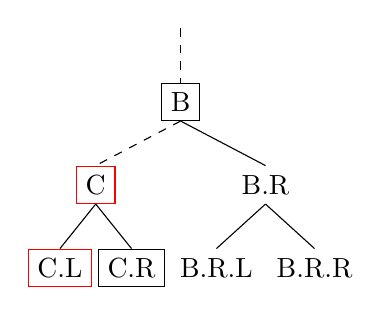
\begin{tikzpicture}[
            roug/.style={draw=red}, roug/.default=,
            noir/.style={draw=black}, noir/.default=,
            leaf/.style={circle, draw}, leaf/.default=,
        ]
        % [grow=right]
        \Tree [\edge[dashed];
        [.\node[noir]{B}; \edge[dashed];
        [.\node[roug]{C}; \node[roug]{C.L}; \node[noir]{C.R}; ]
        [.B.R B.R.L B.R.R ]]]
    \end{tikzpicture}
\end{figure}

\begin{figure}[htbp]
    \centering
    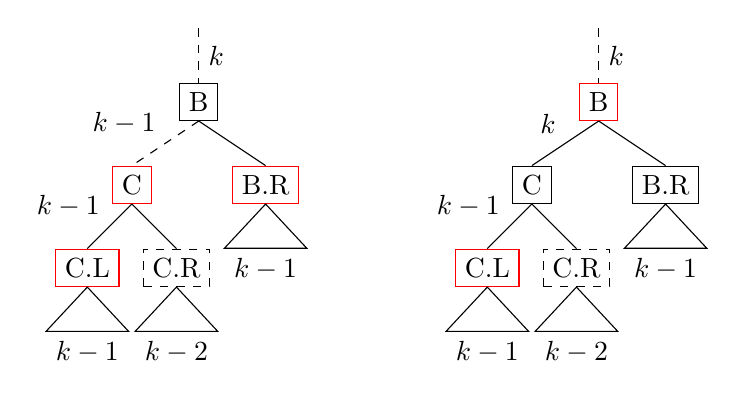
\begin{tikzpicture}[
            roug/.style={draw=red}, roug/.default=,
            noir/.style={draw=black}, noir/.default=,
            noird/.style={draw=black,dashed}, noird/.default=,
            leaf/.style={circle, draw}, leaf/.default=,
        ]
        % [grow=right]
        \Tree [\edge[dashed] node[auto=left]{$k$};
        [.\node[noir]{B};
        \edge[dashed] node[auto=right]{$k-1$};
        [.\node[roug]{C};
        \edge node[auto=right]{$k-1$};
        [.\node[roug]{C.L}; \edge[roof]; {$k-1$} ]
        [.\node[noird]{C.R}; \edge[roof]; {$k-2$} ]]
        [.\node[roug]{B.R}; \edge[roof]; {$k-1$} ]]]
        \begin{scope}[shift={(2in,0in)}]
            \Tree [\edge[dashed] node[auto=left]{$k$};
            [.\node[roug]{B};
            \edge node[auto=right]{$k$};
            [.\node[noir]{C};
            \edge node[auto=right]{$k-1$};
            [.\node[roug]{C.L}; \edge[roof]; {$k-1$} ]
            [.\node[noird]{C.R}; \edge[roof]; {$k-2$} ]]
            [.\node[noir]{B.R}; \edge[roof]; {$k-1$} ]]]
        \end{scope}
    \end{tikzpicture}
\end{figure}

\begin{figure}[htbp]
    \centering
    % \begin{minipage}[b]{0.45\columnwidth}
    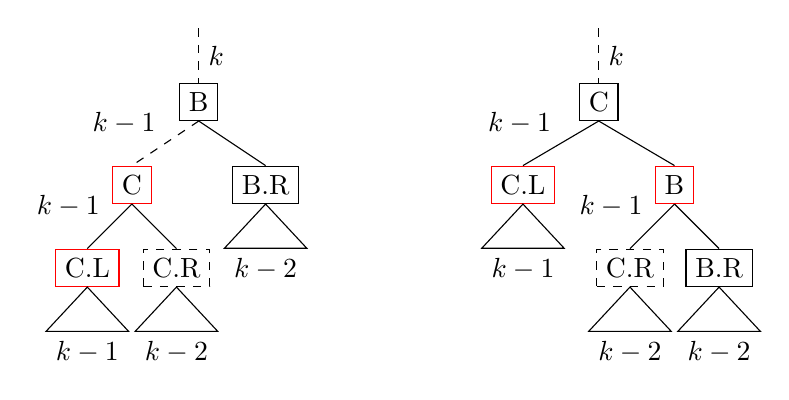
\begin{tikzpicture}[
            edge from parent/.append style={scale=0.4},
            roug/.style={draw=red}, roug/.default=,
            noir/.style={draw=black}, noir/.default=,
            noird/.style={draw=black,dashed}, noird/.default=,
            leaf/.style={circle, draw}, leaf/.default=,
        ]
        % [grow=right]
        \Tree [\edge[dashed] node[auto=left]{$k$};
        [.\node[noir]{B};
        \edge[dashed] node[auto=right]{$k-1$};
        [.\node[roug]{C};
        \edge node[auto=right]{$k-1$};
        [.\node[roug]{C.L}; \edge[roof]; {$k-1$} ]
        [.\node[noird]{C.R}; \edge[roof]; {$k-2$} ]]
        [.\node[noir]{B.R}; \edge[roof]; {$k-2$} ]]]
        \begin{scope}[shift={(2in,0in)}]
            \Tree [\edge[dashed] node[auto=left]{$k$};
            [.\node[noir]{C};
            \edge node[auto=right]{$k-1$};
            [.\node[roug]{C.L}; \edge[roof]; {$k-1$} ]
            [.\node[roug]{B};
            \edge node[auto=right]{$k-1$};
            [.\node[noird]{C.R}; \edge[roof]; {$k-2$} ]
            [.\node[noir]{B.R}; \edge[roof]; {$k-2$} ]]]]
        \end{scope}
    \end{tikzpicture}
\end{figure}
\end{document}